\documentclass{VUMIFPSkursinis}
\usepackage{algorithmicx}
\usepackage{algorithm}
\usepackage{algpseudocode}
\usepackage{amsfonts}
\usepackage{amsmath}
\usepackage{bm}
\usepackage{caption}
\usepackage{color}
\usepackage{float}
\usepackage{graphicx}
\usepackage{listings}
\usepackage{subfig}
\usepackage{wrapfig}

% Titulinio aprašas
\university{Vilniaus universitetas}
\faculty{Matematikos ir informatikos fakultetas}
\department{Programų sistemų katedra}
\papertype{Kursinis darbas}
\title{Interaktyvios pratybos}
\titleineng{Interactive lecture}
\status{3 kurso 2 grupės studentas}
\author{Marijus Siliūnas}
% \secondauthor{Vardonis Pavardonis}   % Pridėti antrą autorių
\supervisor{Dr. Kristina Lapin}
\date{Vilnius – \the\year}

% Nustatymai
% \setmainfont{Palemonas}   % Pakeisti teksto šriftą į Palemonas (turi būti įdiegtas sistemoje)
\bibliography{bibliografija}

\begin{document}
\maketitle

\tableofcontents

\sectionnonum{Įvadas}

\subsectionnonum{Temos aktualumas}
Statistika apie technologijas, dabartinė situacija

\subsectionnonum{Darbo tikslas}
Šiuo darbu siekiama palengvinti darbą dėstytojams paskaitų metu žymint lankomumą. Sukurti sistemą, kurioje studentai skatinami aktyviai dalyvauti paskaitose apdovanojant sistemoje už kiekvieną veiksmą. Atsiskaitymų metu studentams bei dėstytojui aiškiai pateikti atsiskaitomą darbą.
Sukurti sistemą, kuri leistų teikti kokybišką atsaką akivaizdinių studijų užsiėmimų metu, gerina studentų ir dėstytojų bendradarbiavimą.

\subsectionnonum{Siekiami rezultatai}
Ištirti dėstytojų pasikartojantys procesai paskaitų metu ir nustatyta kuriuos iš jų galima automatizuoti. Sukurta sistema su automatizuotu studentų identifikavimo procesu bei studentų skaitinimo aktyviai dalyvauti paskaitoje mechanizmu. 

\section{Studento identifikavimas}

Kuo tai svarbu.

\subsection{Dabartinės situacijos apžvalga}

Užsiėmimų metu yra žymimas studentų lankomumas. Šį darbą atlieka dėstytojas kiekvieno užsiėmimo metu. Studentai kviečiami vardu ir atsiliepę yra pažymimi kaip dalyvaujantys paskaitoje. Taip nereikalingai užimamas paskaitos laikas bei atsiranda žmogiškos klaidos tikimybė. Tai ypač svarbu, kuomet galutinis įvertinimas priklauso ir nuo lankomumo. Dėstytojams tai papildoma atsakomybė ir jie turi patys pasirūpinti priemone, kurioje galėtų vesti studentų lankomumo žurnalą, nes nėra bendros sistemos universitete.  Reikalinga sistema, kurioje būtų suvedami dėstomi dalykai, dėstantys dėstytojai bei studentų grupės ir studentai. Sistemoje būtų vedamas lankomumo žurnalas.

Lankomumo žymėjimą galima visiškai automatizuoti. Taip būtų supaprastinamas dėstytojų darbas bei taupomas laikas. Lankomumo žymėjimą galima automatizuoti ne vienu būdu, tačiau pirmiausia reikia studentus identifikuoti.

\subsection{NFC technologija}
Vienas iš būdų yra Lietuvos studento pažymėjimo (toliau - LSP) panaudojimas studento įdentifikavimui. Naujo pavyzdžio LSP turi integruotą NFC (angl. \textit{Near Field Communication}) technologiją.  Jos pagalba galime nuskaityti LSP unikalų identifikavimo numerį ir pagal jį identifikuoti studentą. Identifikavus studentą sistemoje pažymimas jo dalyvavimas paskaitoje.

Visi studentai pradėję studijuoti įsigyja LSP todėl studentams toks procesas nesukeltų jokių nepatogumų. Norint įgyvendinti tokį identifikavimo procesą dar reikalinga integracija su duomenų baze, kurioje būtų susiejamas unikalus LSP indentifikavimo numeris su LSP duomenimis. Gauti duomenys turėtų būti patikrinami ir su vidine universiteto sistema patikrinant, ar toks studentas tikrai egzistuoja, ar jis turi dalyvauti šioje paskaitoje ir t.t. Taip pat universiteto auditorijose turėtų būti įdiegti NFC skaitytuvai. Norint efektyviai atlikti žymėjimą turėtų būti įrengtas ne vienas, nes pažymėti galima tik po vieną studentą.

\subsection{Bluetooth technologija}
Kitas būdas galėtų būti panaudojant Bluetooth technologiją. Pati technologija nėra nauja, tačiau vis tobulinama. Beveik visi šiuo metu naudojami mobilieji telefonai turi integruotą šią technologiją. Mobiliuosius telefonus turi visi studentai. Kiekvienas įrenginys, kuriame yra integruota Bluetooth technologija, turi savo unikalų identifikavimo numerį, kurį galima nuskaityti. Kaip ir prieš tai pateiktu būdu - šį numerį reikėtų susieti su studento informacija. Privalumas prieš LSP skaitymą - nereikia integruoti trečiųjų šalių paslaugų. Identifikaciniai numeriai išsaugomi ir susiejiami su studentu kuriamoje sistemoje.

Universiteto auditorijose taip pat turėtų būti įdiegiami skaitytuvai, kurie nuskaitytų studentų mobiliųjų telefonų unikalius identifikacinius numerius. Tokio skaitytuvo tereikėtų vieno auditorijoje, nes mobiliųjų telefonų siunčiamus signalus Bluetooth ryšius galima nuskaityti visus vienu metu. Nors studentai turėtų įjungti šią technologiją telefone, pats procesas vyktų žymiai efektyviau ir paprasčiau.

\subsection{NFC ar Bluetooth?}
Pateikti būdai turi ir privalumų, ir trūkumų. Visgi tinkamesnis būdas identifikuoti studentus yra pasitelkus Bluetooth technologiją, nes: nepriklausoma nuo trečiųjų šalių paslaugų (services); auditorijose reikia įrengti mažiau skaitytuvų ir / ar greitesnis identifikavimas (nesusidaro eilės prie skaitytuvų).

\subsection{Mobilioji programėlė studentams}
Toks proceso įgyvendinimas prasideda nuo programėlės sukūrimo išmaniesiems telefonams. Taip pat svarbu, kad programėlė ne tik padėtų identifikuoti studentą, tačiau būtų kuo paprastesnė (reikėtų atlikti kuo mažiau veiksmų) naudotojui.

Kiekvienas įrenginys turintis integruotą Bluetooth technologiją turi ir unikalų MAC (angl. \textit{Media Access Control}) adresą, dar vadinamą fiziniu adresu. Kadangi šis adresas kievienam įrenginiui yra unikalus, tai juo galime naudotis norint identifikuoti studentus. Norint susieti studento mobilųjį telefoną su jo paskyra sistemoje studentas įsidiegia programėlę. Programėlėje studentas prisijungia prie savo paskyros ir susieja mobilųjį telefoną. Programėlė nuskaito telefono Bluetooth MAC adresą ir kartu su studento identifikavimo numeriu (gaunamas prisijungus prie paskyros) siunčia į sistemą. Sistema gautą MAC adresą priskiria tam studentui. Programėlės pagrindinė funkcija yra susieti telefoną su paskyra. Tuo pačiu galima pateikti studento tvarkaraštį, lankomumo ataskaitą.

Norint, kad sistema galėtų naudotis kuo daugiau studentų, programėlė turi būti palaikoma skirtingose įrenginiuose bei operacinėse sistemose. Pačios populiariausios išmaniųjų įrenginių operacinės sistemos yra \textit{Android} ir \textit{iOS}. Taip pat gana plačiai naudojama \textit{Windows Phone} operacinė sistema.

\subsubsection{Programėlių kūrimas pagal operacinę sistemą}

\subsubsubsection{Android}
Tai yra populiariausia, apie 80 procentų rinkos užimanti \cite{MarketShareByOS}, operacinė sistema. Ši platforma yra atviro kodo ir prižiūrima \textit{Google} kompanijos. \textit{Android} operacinė sistema diegiama į tokių kaip \textit{LG}, \textit{Sony} ir kitų gamintojų išmaniuosius telefonus. Šiai platformai programėlės kuriamos \textit{Java} programavimo kalba. Programavimo aplinkai kūrėjai siūlo nemokamą įrankį \textit{Android Studio} bei pamokų ciklą pirmąjai programėlei sukurti.

\subsubsubsection{iOS}
Antra pagal populiarumą, apie 15 procentus rinkos turinti \cite{MarketShareByOS}, operacinė sistema. Ši platforma yra palaikoma ir sukurta \textit{Apple} korporacijos. Programėlės kuriamos \textit{Objective-C} arba \textit{Swift} programavimo kalbomis.

\subsubsubsection{Windows Phone}
Trečia pagal populiarumą, apie 3 procentus išmaniųjų įrenginių rinkos užimanti \cite{MarketShareByOS}, operacinė sistema. Tai yra \textit{Microsoft} korporacijos produktas. Operacinė sistema diegiama \textit{Nokia} korporacijos \textit{Lumia} išmaniųjų telefonų linijoje. Programavimo kalba - \textit{C\#}.

\subsubsection{Viena programėlė - visoms operacinėms sistemoms}
Dažnai poreikis yra palaikyti kuo daugiau įrenginių. Ir šiuo atveju - reikalinga, kad naudojimąsis sistema būtų kuo prieinamesnis. Būtent dėl šios priežasties buvo pradėtos kurti technologijos leisiančios rašyti vieną kodą vienai programėlei ir ji veiktų populiariausiose išmaniųjų įrenginių operacinėse sistemose. Kol kas nėra tiek išvystyta technologija, tačiau šiuo metu galime su nedidelėmis korekcijomis sukurti programėlę tinkamą populiariausioms išmaniųjų irenginių operacinėms sistemoms.

\subsubsubsection{Sava programėlė}

Sparčiai tobulėjanti platforma, skirta kurti programėles \textit{Android}, \textit{iOS} ir \textit{Windows Phone} operacinėms sistemoms, tai \textit{Xamarin} \cite{xamarin}. Naudojantis šia platforma galima kurti visoms trims mobiliosioms operacinėms sistemoms savas (angl. \textit{native}) programėles. Šiuo atveju programėlės yra rašomos \textit{C\#} programavimo kalba, o programinė įranga, reikalinga surinkti bei vystyti programėles, yra nemokama. Vidutiniškai 75 procentai programėlės kodo yra naudojama bendrai tarp operacinių sistemų. Platforma suteikia pilną priėjimą prie įrenginio operacinės sistemos aplikacijų programavimo sąsajos (visose operacinėse sistemose). Vartotojo sąsają galima kurti pagal operacinės sistemos standartus arba naudojant platformos kūrėjų įrankį \textit{Xamarin.Forms}.

\subsubsubsection{Saityno programėlė}

Priklausomai nuo poreikių, galima sukurti tinklalapį pritaikytą mobiliesiems įrenginiams. Kuriant galima pasitelkti karkasus, skirtus kurti būtent tokias saityno programėles. Tai yra greitas ir pigus būdas, prieinamas iš visų operacinių sistemų, tačiau tinkamas tik tuomet, kai nereikia arba reikalingos elementarios (garsas, failai įrenginio atmintyje) sąsajos su įrenginiu. Dėl to šis variantas nėra tinkamas mūsų atveju - nėra galimybės pasinaudoti įrenginio \textit{Bluetooth} ryšiu.

\subsubsubsection{Hibridinė programėlė}

Hibridinė programėlė - tai saityno programėlė, tačiau integruota į 	savą programėlę. Tai suteikia galimybę priėjimą prie įrenginio operacinės sistemos aplikacijų programavimo sąsajos (angl. \textit{Application Programming Interface, API}). Tokiu būdu mes galime pasiekti išmaniojo įrenginio resursus, o šiuo atveju - mums reikalingą \textit{Bluetooth} modulį.

Vienas iš labiausiai paplitusių karkasų yra \textit{Ionic} \cite{hybridFrameworks}. Naudojantis šiuo karkasu galime programėlę kurti kaip tinklalapį, programuojant \textit{JavaScript} programavimo kalba bei rašant \textit{HTML} ir \textit{CSS} kodą vartotojo sąsajai kurti.

\subsubsubsection{Hibridinė ar sava programėlė?}

Tiek vienas, tiek kitas programėlių kūrimo būdas turi ir pliusų, ir minusų. Hibridines programėles galima kurti greičiau ir paprasčiau, tačiau jų veikimo sparta bei vientisumas gali kelti nepatogumų naudotojams. Taip pat yra sudėtingiau išnaudoti įrenginio ir jo operacinės sistemos teikiamas funkcijas, pasiekiamas per aplikacijų programavimo sąsaja. Vis dėlto tai yra geresnis variantas nei rašyti kiekvienai operacinei sistemai atskirą programėlę, laiko ir kainos atžvilgiu.

Kuriamos sistemos realizacijai reikia kuo geresnės integracijos su išmaniuoju įrenginiu. Todėl tinkamiausias būdas kurti programėlę sistemai yra naudojant \textit{Xamarin} platformą. Ji leis sukurti intuityvesnę, vientisesnę bei patikimesnę programėlę.

\subsubsection{Programėlės vartoto sąsaja}

Studentams skirtos programėlės pagrindinės funkcijos - pasižymėti dalyvavimą užsiėmime bei susieti įrenginį su paskyra. Projektuojant vartotojo sąsają pagrindinis dėmesys skiriamas šių veiksmų paprastumui, stengiamasi, kad užduočių atlikimui reikėtų kuo mažiau veiksmų.

Vartotojo sąsaja kuriama naudojant \textit{Xamarin Forms} įrankį, todėl visuose įrenginiuose, nepriklausomai nuo operacinės sistemos, vartotojo sąsaja bus atvaizduojama ta pati. Šio įrankio naudojimas pagreitina įgyvendinimą, nes nebereikia atskirai kurti kiekvienai operacinei sistemai vartotojo sąsajos atskirai. Tuo pačiu reikia atsižvelgti į tai, jog dėl tos pačios priežasties įrenginių ekrano dydžiai labai skirtingi.

\begin{figure}[H]
	\centering
	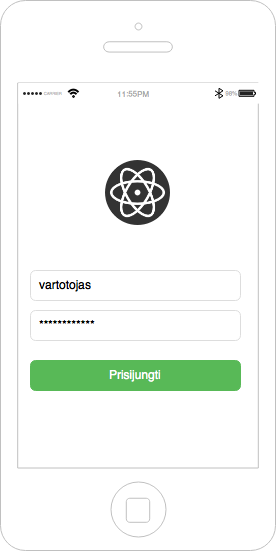
\includegraphics[scale=0.5]{img/kursinio_app_login}
	\caption{Prisijungimo langas}
	\label{img:loginView}
\end{figure}

Prisijungimo langas (\ref{img:loginView} pav.) matomas tik pirmą kartą prisijungiant arba po atsijungimo. Naudotojui reikia suvesti prisijungimo vardą bei slaptažodį ir paspausti mygtuką „Prisijungti“. Jei pateikti duomenys teisingi, atidaromas pagrindinis langas (\ref{img:mainView} pav.). Kitu atveju rodomas klaidos pranešimas.

\begin{figure}[H]
	\centering
	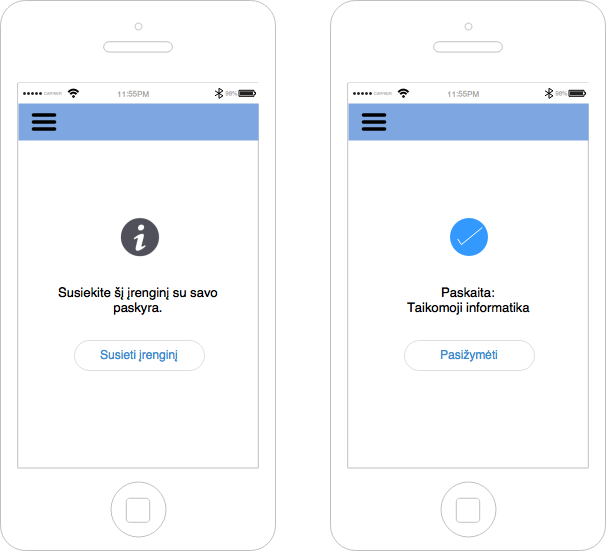
\includegraphics[scale=0.5]{img/kursinio_app_main}
	\caption{Pagrindinis langas}
	\label{img:mainView}
\end{figure}

Pagrindiniame lange (\ref{img:mainView} pav.), priklausomai nuo to, ar esame susieję įrenginį su mūsų paskyra, matome arba pranešimą, kad turime susieti įrenginį su paskyra arba paskaita, kurioje galime pasižymėti, kad dalyvaujame.

\begin{figure}[H]
	\centering
	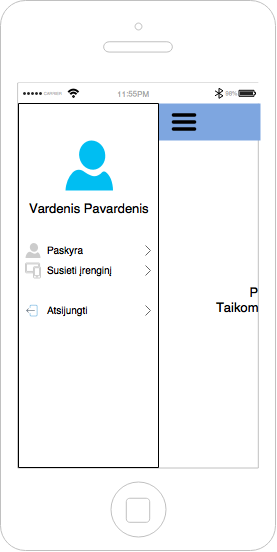
\includegraphics[scale=0.5]{img/kursinio_app_menu}
	\caption{Meniu}
	\label{img:menuView}
\end{figure}

Meniu (\ref{img:menuView} pav.) pateikiamas prisijungusio naudotojo vardas ir pavardė bei nedidelė profilio nuotrauka. Meniu atidaryti galima viršutinėje juostoje paspaudus meniu ikoną.

\subsubsection{Programėlės naudojimo scenarijai}

\subsubsubsection{Prisijungimas}

Įdiegus ir pirmą kartą programėlę paleidus naudotojui atidaromas prisijungimo langas (\ref{img:loginView} pav.). Studentas suveda prisijungimo vardą bei slaptažodį. Spaudžia prisijungti. Sistemai grąžinus sėkmingą pranešimą, programėlė išsisaugo prisijungimo duomenis (arba grąžintą access token, priklausomai nuo sistemos įgyvendinimo). Kitą kartą paleidus programėlę prisijungimas vyksta automatiškai.

\subsubsubsection{Įrenginio susiejimas}

Pagrindiniame programėlės lange (\ref{img:mainView} pav.) matome pranešimą, kad nėra susietas įrenginys su paskyra. Spaudžiame „Susieti įrenginį“. Programėlė surenka reikalingą informaciją apie įrenginį (\textit{Bluetooth MAC} adresą) ir siunčia užklausą į sistemos aplikacijų programavimo sąsają. Grąžinama žinutė apie sėkmingą arba nesėkmingą įrenginio susiejimą su paskyra.

\textbf{Alternatyvus scenarijus:} Prisijungus programėlėje, atidarome meniu (\ref{img:menuView} pav.) paspausdami ant meniu ikonos viršutinėje juostoje. Atsidariusiame meniu pasirenkame „Susieti įrenginį“.

\subsubsubsection{Lankomumo pasižymėjimas}

Studentas atėjęs į paskaitą įsijungia programėlę bei įrenginio Bluetooth ryšį. Pagrindiniame lange (\ref{img:mainView} pav.) spaudžia mygtuką „Pasižymėti“. Programėlė ieško skaitytuvo ir nuskaito jo siunčiamą informaciją: paskaitos pavadinimą, dėstytojo vardą ir pavardę. Rodomas patvirtinimo langas su šia informacija. Studentas spaudžia „Taip“. Patvirtinimas siunčiamas į sistemą ir pažymimas studento dalyvavimas paskaitoje.

\textbf{Alternatyvus scenarijus:} Studentui tereikia įjungti Bluetooth ryšį ir būti susiejus įrenginį su paskyra. Skaitytuvas aptikęs įrenginį automatiškai pažymi studento dalyvavimą paskaitoje.

\subsubsubsection{Paskyros peržiūra}

Programėlėje studentas taip pat gali peržiūrėti savo paskyrą meniu (\ref{img:menuView} pav.) spausdamas mygtuką „Paskyra“.

\subsection{Skaitytuvas - išmanusis telefonas}
Kitas svarbus komponentas, norint identifikuoti studentus, naudojant \textit{Bluetooth} ryšį - skaitytuvas. Tai galėtų būti atskiras prietaisas arba tiesiog išmanusis telefonas. Reikalinga sukurti atskirą programėlę, kuri būtų įdiegta dėstytojo išmaniajame telefone.

Paskaitos metu programėlė nuskaito įrenginius esančius patalpoje ir siunčia įrenginių sąrašą su jų \textit{Bluetooth MAC} adresais į sistemą, kur gautas unikalus identifikatorius susiejamas su studento paskyra ir pažymimas jo dalyvavimas paskaitoje. Norint tai įgyvendint, dėstytojas taip pat turi turėti savo paskyrą sistemoje. Paskyroje pridedamos paskaitos, priskiriamos grupės bei studentai.

Kaip ir programėlė skirta studentams, taip ir skirta dėstytojams turi būti kuo prieinamesnė. Todėl jos kūrimui taip pat pasirinkta \textit{Xamarin} platforma.

\subsubsection{Skaitytuvo programėlės vartotojo sąsaja}

\subsubsection{Skaitytuvo programėlės funkcijos}

\subsubsubsection{Prisijungimas}

Įdiegus ir pirmą kartą programėlę paleidus naudotojui atidaromas prisijungimo langas. Dėstytojas suveda prisijungimo vardą bei slaptažodį. Spaudžia prisijungti. Sistemai grąžinus sėkmingą pranešimą, programėlė išsisaugo prisijungimo duomenis arba prieigos raktą (priklausomai nuo sistemos vidinės pusės įgyvendinimo). Kitą kartą paleidus programėlę prisijungimas vyksta automatiškai.

\subsubsubsection{Paskaitos pradžia}

Paleidus programėlę ir prisijungus (automatiškai arba suvedus prisijungimo duomenis) pagrindiniame lange spaudžia „Pradėti paskaitą“. Atidaromas paskaitų sąrašas, rikiuotas pagal paskaitos laiką (nurodoma administravimo dalyje). Paspaudžia ant paskaitos, atsiranda patvirtinimo langas, spaudžia „Pradėti“. Programėlė pradeda skleisti informaciją \textit{Bluetooth} ryšiu. Rodomas paskaitos langas su pasižymėjusiais studentais.

\textbf{Alternatyvus scenarijus:} Pradėjus paskaitą periodiškai ieškoma įrenginių su įjungtu \textit{Bluetooth} ryšiu. Rastų įrenginių \textit{Bluetooth MAC} adresai siunčiami į sistemą.

\subsubsubsection{Paskaitos pabaiga}

Paskaitos lange spaudžia „Užbaigti paskaitą“. Rodomas patvirtinimo pranešimas, spaudžia „Užbaigti“. Programėlė nusiunčia užklausą į sistemą dėl paskaitos užbaigimo. Rodomas pranešimas su sėkmingo arba nesėkmingo užbaigimo tekstu. Atidaromas pagrindinis langas.

\section{Sistemos vidinė pusė}

Apžvelgėme, kokiu būdu ir kokiomis priemonėmis sistemos naudotojai galės naudotis sistema. Bet visa tai neveiks be pagrindinės sistemos dalies. Kaip pavadinti backend? API?

\subsection{Programų sąsaja}

Visas bendravimas tarp klientų (mobiliųjų programėlių, web?) ir sistemos vyksta per aplikacijų programavimo sąsają.

\subsubsection{Saugumas}

Generuojami tokenai, klientuose nesaugomi prisijungimo duomenys. Payload su encryption? Pasiklausti Eligijaus apie šitą.

\subsection{Administravimo aplinka}



\sectionnonum{Rezultatai ir išvados}
Rezultatų ir išvadų dalyje turi būti aiškiai išdėstomi pagrindiniai darbo
rezultatai (kažkas išanalizuota, kažkas sukurta, kažkas įdiegta) ir pateikiamos
išvados (daromi nagrinėtų problemų sprendimo metodų palyginimai, teikiamos
rekomendacijos, akcentuojamos naujovės).

\printbibliography[heading=bibintoc]  % Šaltinių sąraše nurodoma panaudota
% literatūra, kitokie šaltiniai. Abėcėlės tvarka išdėstomi darbe panaudotų
% (cituotų, perfrazuotų ar bent paminėtų) mokslo leidinių, kitokių publikacijų
% bibliografiniai aprašai.  Šaltinių sąrašas spausdinamas iš naujo puslapio.
% Aprašai pateikiami netransliteruoti. Šaltinių sąraše negali būti tokių
% šaltinių, kurie nebuvo paminėti tekste.

% \sectionnonum{Sąvokų apibrėžimai}
\sectionnonum{Santrumpos}
Sąvokų apibrėžimai ir santrumpų sąrašas sudaromas tada, kai darbo tekste
vartojami specialūs paaiškinimo reikalaujantys terminai ir rečiau sutinkamos
santrumpos.

\appendix  % Priedai
% Prieduose gali būti pateikiama pagalbinė, ypač darbo autoriaus savarankiškai
% parengta, medžiaga. Savarankiški priedai gali būti pateikiami ir
% kompaktiniame diske. Priedai taip pat numeruojami ir vadinami. Darbo tekstas
% su priedais susiejamas nuorodomis.

\end{document}
